\section{System Overview}
We introduced a location based evolving passwords scheme into the 802.11i protocol with pre-shared key mode to provide fine-grained access control and high security for WLAN. But just as significantly, introducing of evolving passwords scheme will not put extra burdens on administrators and users. To join WLAN, mobile devices must share the same password with APs at the same time, or they cannot pass APs’ authentication. However, we make passwords evolve at short intervals. A long random number is used to update passwords. It is called physical parameter because it can only be obtained in a constrained location protected by physical access controls for mobile devices. Once APs update their passwords, mobile devices should always synchronize their own passwords with APs’. To update passwords, mobile devices have to pass physical access controls and gain physical parameters. Users who are told old passwords but cannot continue to pass physical access controls will be rejected to join WLAN. That is, users’ WLAN authorization is revoked implicitly. 

As is shown in the following graph, the location based passwords evolving system consists of three parts: a special device called physical generator update physical parameters and drive passwords evolving process, one or more APs whose passwords evolve automatically at set intervals, and one or more mobile devices which are able to synchronize passwords with APs automatically when necessary and possible. 
\begin{figure}
	\begin{center}
		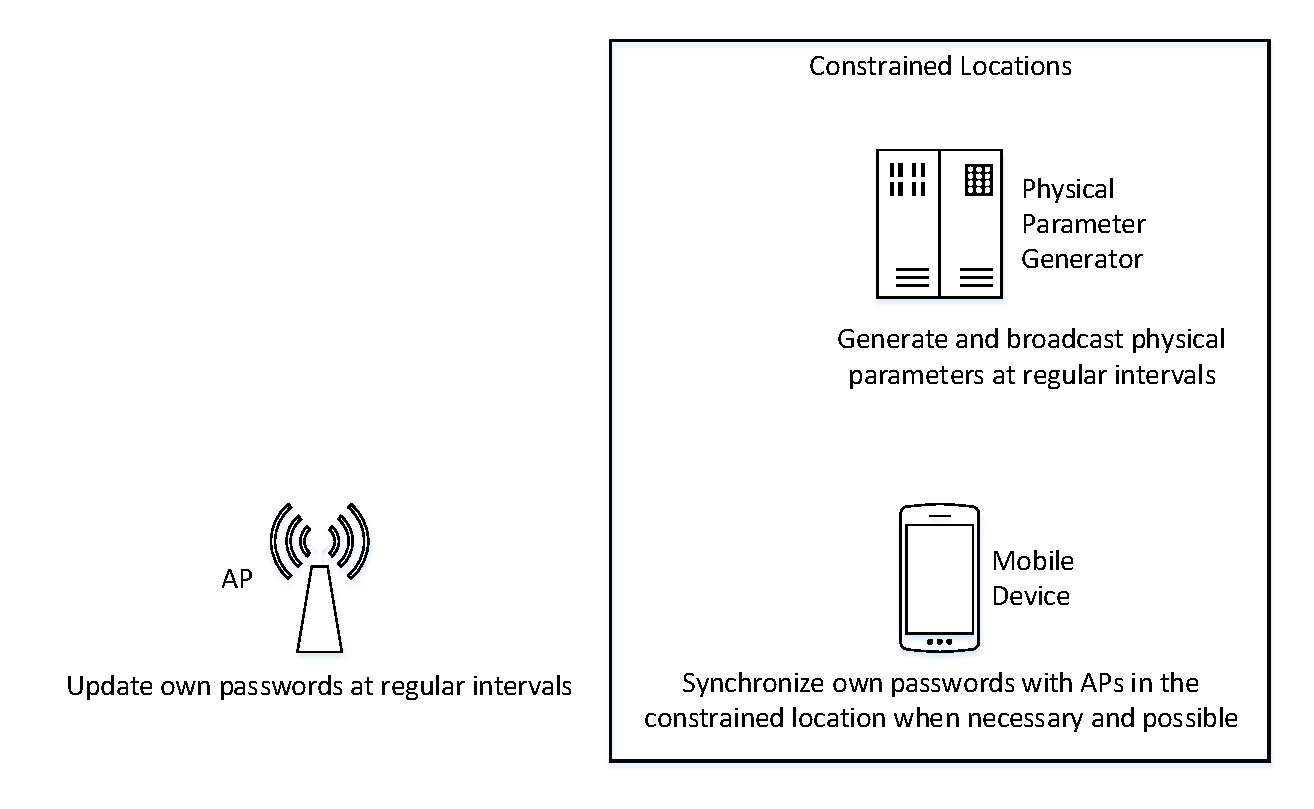
\includegraphics[width=\textwidth]{System_Overview.pdf}
		\caption{Overview of the Proposed System}
		\label{Fig:3.1}
	\end{center}
\end{figure}

At most of the time, APs and mobile devices share the same password. APs’ initial passwords are set by administrators while mobile devices’ initial passwords are obtained through an out-of-band way. When passwords evolves, both APs and mobile devices can get the same new passwords on the basis of the same old passwords and physical parameters. The passwords evolving process is simple. The passwords evolving process of each AP and each mobile devices is independent of each other. At the set update interval, 
\begin{itemize}
	\item the physical parameter generator will generate new physical parameters and broadcasts them to a constrained location protected by physical access controls; 
	\item APs get new physical parameters though a secure channel and update their own passwords; 
	\item if users pass physical access controls and enter the constrained location, mobile devices can get new physical parameters and update their own passwords by the same way with APs. 
\end{itemize}
A successful password update process enables mobile devices to join WLAN in the new passwords evolving interval. Mobile devices are able to join WLAN continuously until they do not enter the specific location in a whole passwords evolving interval. 
